\FloatBarrier

\begin{figure}[h!]
	\centering
	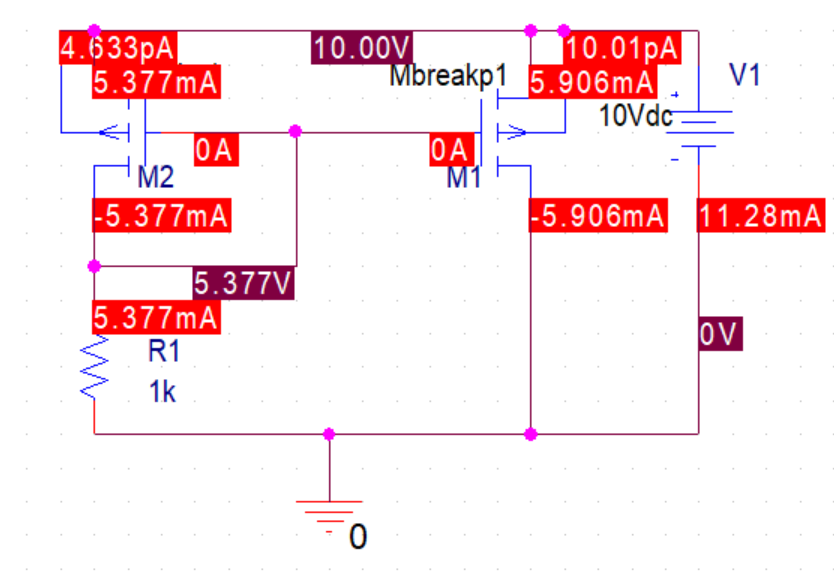
\includegraphics[scale=0.75]{../images/circuit1_bp.PNG}
	\caption{PMOS Current Mirror Bias Simulation}
	\label{fig:circuit1_bp}
\end{figure}

\FloatBarrier

A current mirror takes an input current $i_{in}$ and produces an output current $i_{out}$ such that $i_{in} \approx i_{out}$.
However, looking at figure (\ref{fig:circuit1_bp}), which current, whether it is the current through $M_2$ or $M_1$, is $i_{in}$ or $i_{out}$ is ambiguous.
In order to determine which is truly the input current, a known current must be supplied through one transistor.

\FloatBarrier

\begin{figure}[h!]
	\centering
	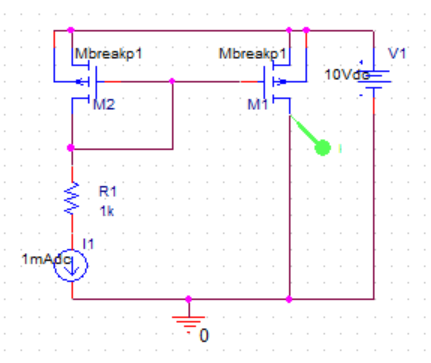
\includegraphics[scale=0.75]{../images/thought_exp1.PNG}
	\caption{Known Current Supplied to $M_2$}
	\label{fig:thought_exp1}
\end{figure}

\FloatBarrier

\FloatBarrier

\begin{figure}[h!]
	\centering
	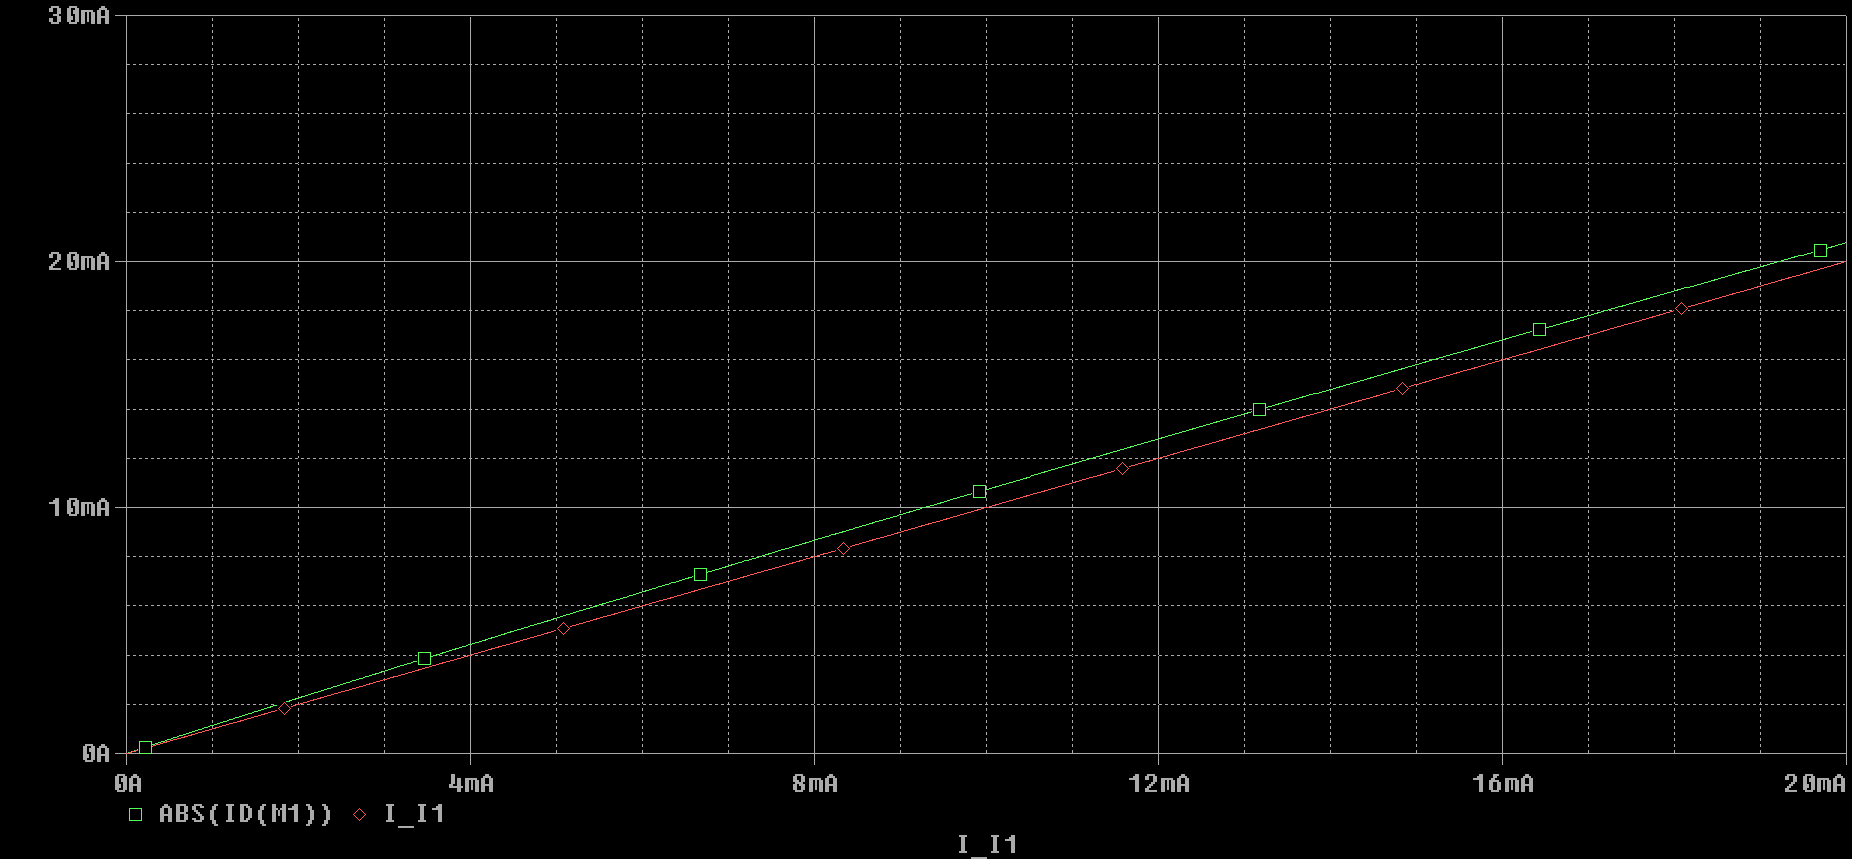
\includegraphics[scale=0.50]{../images/plot_1.PNG}
	\caption{$i_{M2}$ versus $i_{M1}$}
	\label{fig:plot_1}
\end{figure}

\FloatBarrier

{\footnotesize The green line is $i_{M1}$, and the red line is $i_{M2}$. They are plotted against the known current $i_{M2}$.}

\FloatBarrier

Across a range of current, $i_{M1} \approx i_{M2}$ when $i_{M2}$ is the known current.
Suppose that $i_{M1}$ is fixed instead.

\FloatBarrier

\begin{figure}[h!]
	\centering
	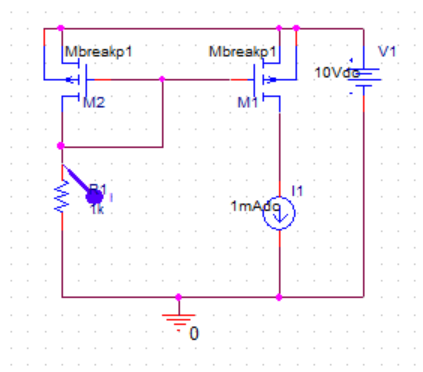
\includegraphics[scale=0.75]{../images/thought_exp2.PNG}
	\caption{Known Current Supplied to $M_1$}
	\label{fig:thought_exp2}
\end{figure}

\FloatBarrier

\FloatBarrier

\begin{figure}[h!]
	\centering
	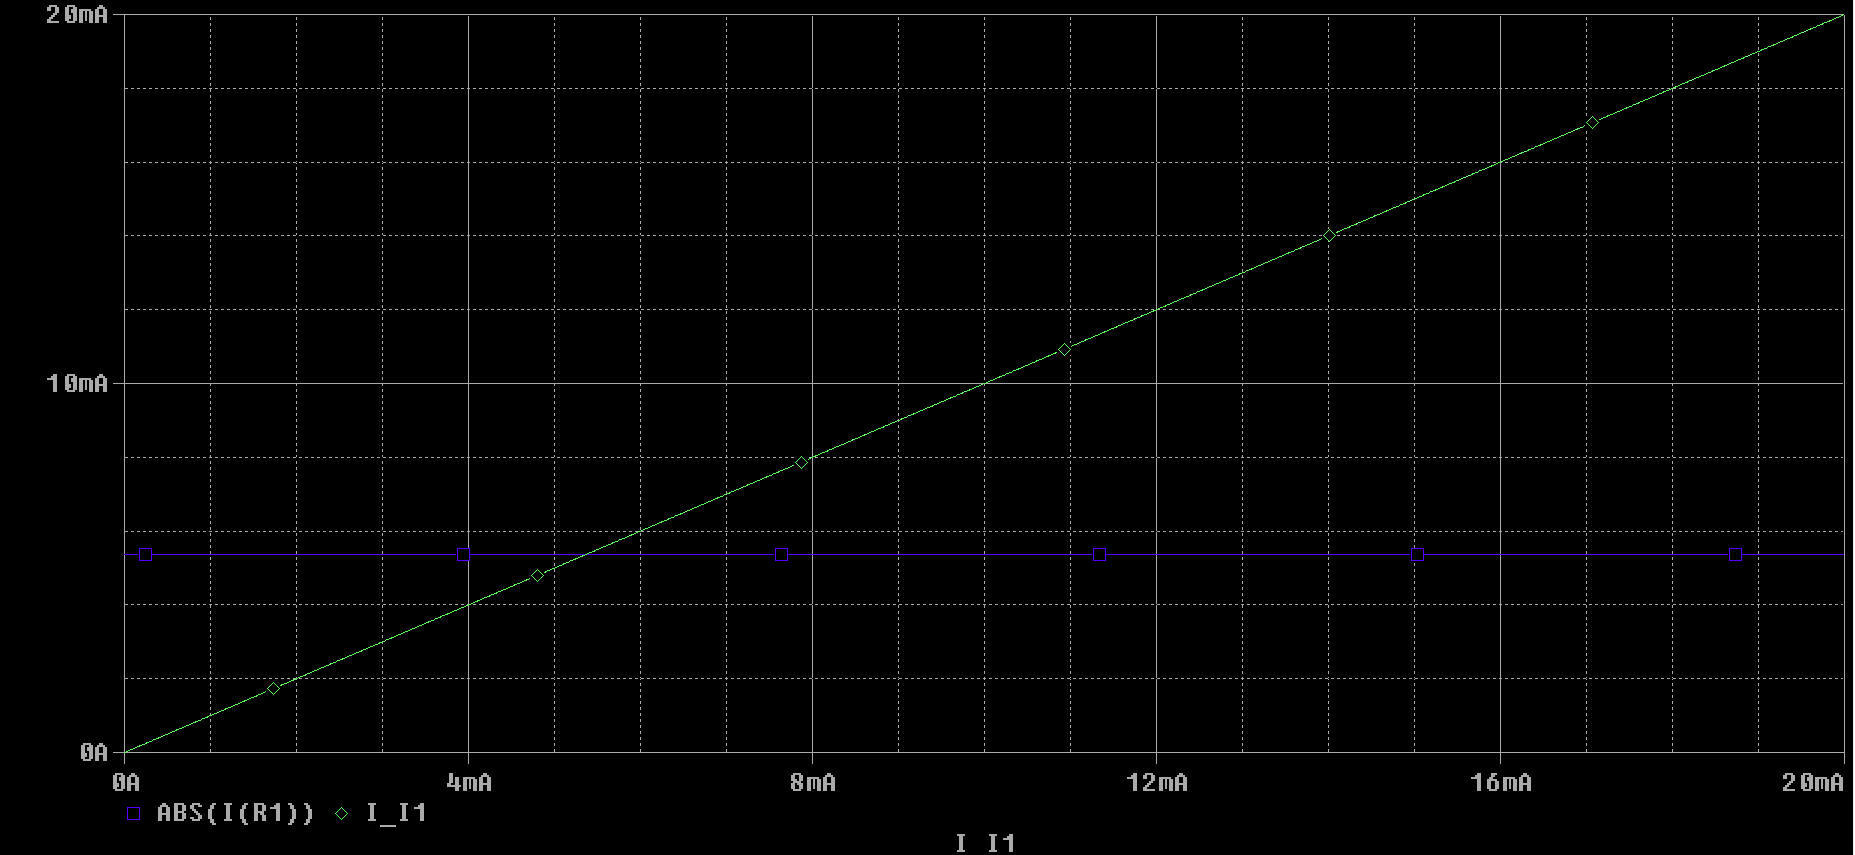
\includegraphics[scale=0.50]{../images/plot_2.PNG}
	\caption{$i_{M1}$ versus $i_{M2}$}
	\label{fig:plot_2}
\end{figure}

\FloatBarrier

{\footnotesize The green line is $i_{M1}$, and the blue line is $i_{M2}$. They are plotted against the known current $i_{M1}$.}

Here, $i_{M2}$ remains constant, regardless of the value of $i_{M1}$.
Therefore, setting the value of $i_{M2}$ determines the value of $i_{M1}$, but setting the value of $i_{M1}$ has no effect on the value of $i_{M2}$.
So, the current through the transistor $M_2$ is the input current being mirrored ($5.377$\si{\milli\ampere}), and the current through the transistor $M_1$ is the output current that mirrors $i_{M2}$.

\FloatBarrier

\begin{figure}[h!]
	\centering
	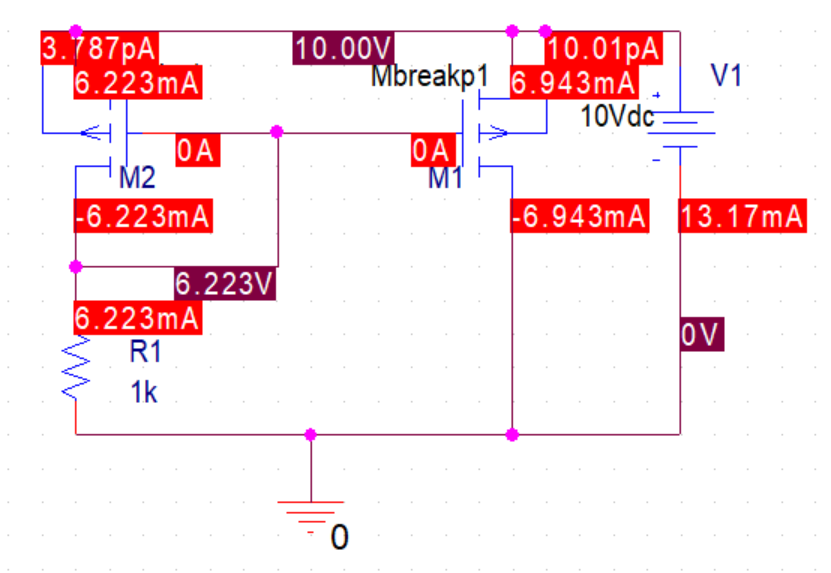
\includegraphics[scale=0.75]{../images/double_width_means_double_current.PNG}
	\caption{Doubling the Width of the MOSFETs}
	\label{fig:double_width_means_double_current}
\end{figure}

\FloatBarrier

Suppose the width of each transistor, $M_1$ and $M_2$, is doubled.
More current flows through each transistor.
Widening transistors allows more charge to flow through a given channel in a fixed time interval. 
So, $6.223$\si{\milli\ampere} is the new current value being mirrored.

\FloatBarrier

\begin{figure}[h!]
	\centering
	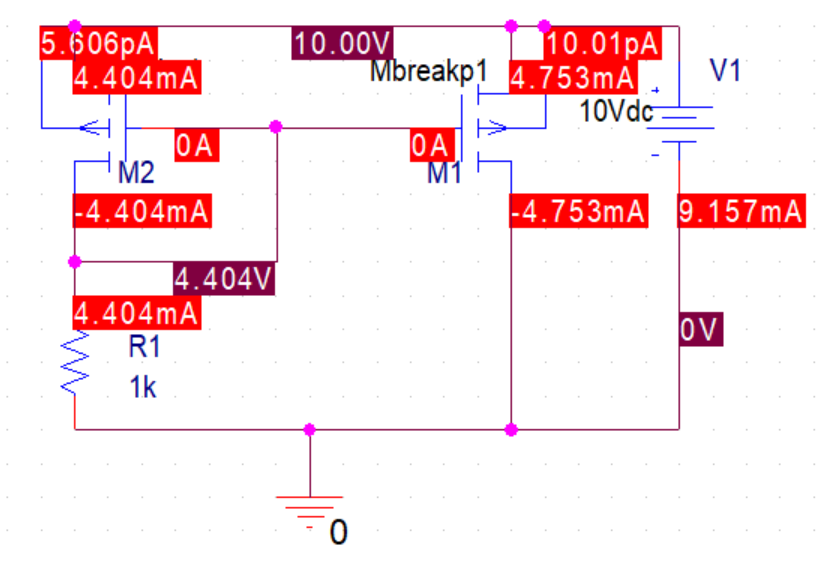
\includegraphics[scale=0.75]{../images/half_width_means_half_current.PNG}
	\caption{Halving the Width of the MOSFETs}
	\label{fig:half_width_means_half_current}
\end{figure}

\FloatBarrier

If the width of each transistor is now halved, fewer charges are able to flow through a channel per unit time.
So, less current flows through each transistor.
$4.404$\si{\milli\ampere} is the new current value being mirrored. \\

Table (\ref{tab:mirrored_currents}) presents the mirrored current values at different $\frac{W}{L}$ ratios.
Clearly, increasing $\frac{W}{L}$ for the transistors increases the mirrored current values because of the mechanics described above, namely that wider channels allow more charges to flow per unit time, leading to more current ceteris paribus.

\FloatBarrier

\begin{table}[h!]
	\centering
	\caption{$i_{in}$ at Various $\frac{W}{L}$ Values}
	\label{tab:mirrored_currents}
	\csvautotabular{../tables/mirrored_currents.csv}
\end{table}

\FloatBarrier
